\documentclass[12pt]{article}

\usepackage[utf8x]{inputenc} % Включаем поддержку UTF8  
\usepackage[russian]{babel}  % Включаем пакет для поддержки русского языка  
\usepackage{hyperref}        % Для гиперссылок

% Математика
\usepackage{amsmath}         % В т.ч. для матриц
\usepackage{amssymb}

% Прога
\usepackage{etoolbox}
\usepackage{listings}

% Цвета
\usepackage{xcolor}

% Картинки
\usepackage{graphicx}
\graphicspath{ {./images/} }

\newtheorem{property}{Свойство}
\newtheorem{consequence}{Следствие}[property]

\newcommand{\qedsymbol}{\rule{2mm}{2mm}}

\begin{document}

\thispagestyle{empty}
\begin{center}
\textbf{ПРАВИТЕЛЬСТВО РОССИЙСКОЙ ФЕДЕРАЦИИ}

\vspace{5ex}
	
\textbf{Федеральное государственное автономное образовательное учреждение \\ высшего образования \\ <<Национальный исследовательский университет \\ <<Высшая школа экономики>>}
\end{center}
\vspace{5ex}

\begin{center}
    Московский институт электроники и математики им. А.Н. Тихонова  
    
    \vspace{5ex}
    
    Департамент прикладной математики
    
    \vspace{10ex}
    \textbf{Отчёт \\ по лабораторной работе №6 \\ по курсу <<Алгоритмизация и программирование>>}
	\vspace{7ex}

\end{center}

\begin{center} 
\begin{tabular}{| p{0.3\linewidth}| p{0.3\linewidth}| p{0.3\linewidth}|}
 \hline	
ФИО студента & Номер группы & Дата \\  \hline
 & & \\  
Вязов Глеб \newline Дмитриевич & БПМ-231 & 16.12.2023\\  
 & & \\  \hline		
\end{tabular}
\end{center}

\begin{center}
	\vspace{3ex}
	
	\vfill
   
   \normalsize
    
	\textbf{Москва, 2023}
\end{center}

\newpage

%---------------------------------------------------------------------------------

\section*{Задание (вариант №7)}
Размер динамического массива вводится пользователем на этапе выполнения. Тип
массива указан в задании. Элементы массива вводятся с клавиатуры. Написать функции
заполнения массива и вывода массива. Написать функцию модификации массива
указанных элементов. Вспомогательные массивы не использовать.

Тип массива -- double. Удалить все положительные элементы, расположенные между первым
максимальным и последним минимальным элементами.

\newpage

%---------------------------------------------------------------------------------

\section*{Решение}\addcontentsline{toc}{section}{Решение}

\lstset{ %
texcl=true,%
language=C,                 % выбор языка для подсветки
basicstyle=\small\sffamily, % размер и начертание шрифта для подсветки кода
numbers=left,               % где поставить нумерацию строк (слева\справа)
numberstyle=\tiny,           % размер шрифта для номеров строк
stepnumber=1,                   % размер шага между двумя номерами строк
numbersep=5pt,                % как далеко отстоят номера строк от подсвечиваемого кода
backgroundcolor=\color{white}, % цвет фона подсветки - используем \usepackage{color}
showspaces=false,            % показывать или нет пробелы специальными отступами
showstringspaces=false,      % показывать или нет пробелы в строках
showtabs=false,             % показывать или нет табуляцию в строках
frame=single,              % рисовать рамку вокруг кода
tabsize=3,                 % размер табуляции по умолчанию равен 2 пробелам
captionpos=t,              % позиция заголовка вверху [t] или внизу [b] 
breaklines=true,           % автоматически переносить строки (да\нет)
breakatwhitespace=false, % переносить строки только если есть пробел
escapeinside={\%*}{*)},   % если нужно добавить комментарии в коде
inputencoding=utf8x,
extendedchars=\true
}

\begin{lstlisting}[label=string_code1,caption=C]
#include <stdio.h>
#include <stdlib.h>

// Функция возвращает индекс первого максимального элемента
int first_max_index(double *array, int k) {
    double max = array[0];
    int max_index = 0;

    for (int i=1; i<k; i++) {
        if (array[i] > max) {
            max = array[i];
            max_index = i;
        }
    }

    return max_index;
}

// Функция возвращает индекс последнего минимального элемента
int last_min_index(double *array, int k) {
    double min = array[0];
    int min_index = 0;

    for (int i=1; i<k; i++) {
        if (array[i] <= min) {
            min = array[i];
            min_index = i;
        }
    }

    return min_index;
}

// Функция сдвигает элементы на один влево, начиная с index
void move_elements(double *array, int k, int index) {
    for(int i=index; i<k-1; i++) {
        array[i] = array[i + 1];
    }
}

// Функция удаляет элементы
// Возвращает указатель на новое место в памяти
double* delete(double *array, int k, int* new_size) {
    int first = first_max_index(array, k);
    int last = last_min_index(array, k);
    int count_delete_elements = 0;
    // Если первый индекс указывает на один из двух последних элементов (k-1 или k-2)
    // Или последний индекс указывает на один из двух первыв элементов (0 или 1)
    // То в этом массиве ничего удалять не нужно
    if (first >= k-2 || last <= 1) {
        *new_size = k;
        return array;
    }

    int index = first+1;
    while (index < last) {
        if (array[index] <= 0) {
            index++;
            continue;
        }

        move_elements(array, k, index);
        last--;
        count_delete_elements++;
    }

    *new_size = k - count_delete_elements;
    array = realloc(array, (*new_size) * sizeof(double));
    return array;
}

// Выделение памяти для массива из k элементов
double* get_memory(int* k) {
    printf("Введите длину массива: ");
    scanf("%d", k);

    // Выделение памяти для k элементов, размерности sizeof(double)
    // И инициализируем всё нулями
    double *array = calloc(*k, sizeof(double));
    return array;
}

// Заполнение массива, длиной k, вещественными элементами
double * create_array(double *array, int k) {
    for (int i=0; i<k; i++) {
        scanf("%lf", &array[i]);
    }
    return array;
}

// Вывод массива длиной k с вещественными элементами
void print_array(double *array, int k) {
    for (int i=0; i<k; i++) {
        printf("%10.4lf\t", array[i]);
    }
}

int main() {
    // Меняем кодировку на UTF-8, чтобы можно было писать на русском
    system("chcp 65001");
    // Ввод переменных. Дружественный интерфейс
    printf("Выполнил задание: Вязов Глеб. Группа: БПМ231\n");

    unsigned int k;
    double *array = get_memory(&k);

    // Если память не выделилась -- возвращаем ошибку
    if (array == NULL) {
        return 1;
    }
    create_array(array, k);
    printf("Вы создали массив: ");
    print_array(array, k);

    int new_size = k;
    double* new_array = delete(array, k, &new_size);

    // После realloc память может выделиться некорректно
    if (array == NULL) {
        return 1;
    }

    printf("\nПреобразованный массив: ");
    print_array(new_array, new_size);

    return 0;
}

\end{lstlisting} 

\newpage

%---------------------------------------------------------------------------------

\section*{Тестирование}

\begin{enumerate}

\item \textbf{Тест №1.} 

\textit{Ввод:} 
Длина массива: 5
Элементы массива: 100, 1, 2, 3, -100

\textit{Вывод:} 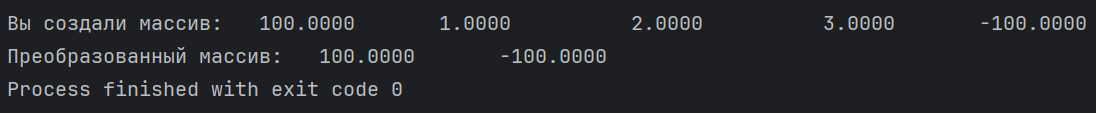
\includegraphics[width=1\textwidth]{img1}



\item \textbf{Тест №2.}

\textit{Ввод:}
Длина массива: 5
Элементы массива: -100, 1, 2, 3, 100

\textit{Вывод:} 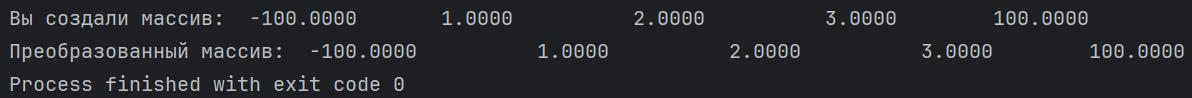
\includegraphics[width=1\textwidth]{img2}



\item \textbf{Тест №3.}

\textit{Ввод:}
Длина массива: 5
Элементы массива: 100, 100, 1, -1, -100

\textit{Вывод:} 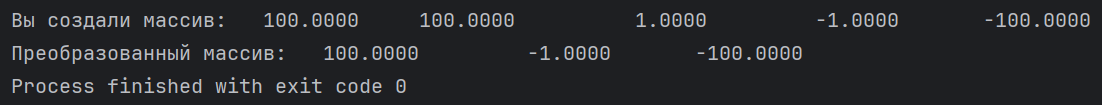
\includegraphics[width=1\textwidth]{img3}


\end{enumerate}


\end{document}
